\documentclass[11pt]{article}
\usepackage[margin=1in]{geometry}
\usepackage{amsmath,amsthm,amssymb}
\usepackage{algorithm2e}
\usepackage{tikz}
\usepackage{xcolor}
\usetikzlibrary{arrows.meta,positioning,shapes.geometric,patterns,decorations.pathreplacing}

% Theorem environments
\newtheorem{example}{Example}[section]
\newtheorem{exercise}{Exercise}[section]
\newtheorem{definition}{Definition}[section]

% Notation
\newcommand{\Bernoulli}[2]{\mathcal{B}^{#2}(#1)}
\newcommand{\Obv}[1]{\widehat{#1}}
\newcommand{\ValidEnc}[1]{\text{ValidEnc}(#1)}

\title{Learning Bernoulli Types and Oblivious Computing:\\A Pedagogical Guide with Graduated Examples}
\author{From Basics to Advanced Concepts}
\date{\today}

\begin{document}
\maketitle

\begin{abstract}
This guide provides a graduated learning path through Bernoulli types and oblivious computing, starting from simple examples and building to complex applications. Each concept is illustrated with visual diagrams, working code, and exercises with solutions.
\end{abstract}

\section{Level 1: Understanding Approximation}

\subsection{The Simplest Bernoulli Type}

\begin{example}[A Coin That's Usually Right]
Imagine a biased coin that shows the correct answer 90\% of the time. This is a Bernoulli Boolean with false negative rate $\beta = 0.1$.

\begin{center}
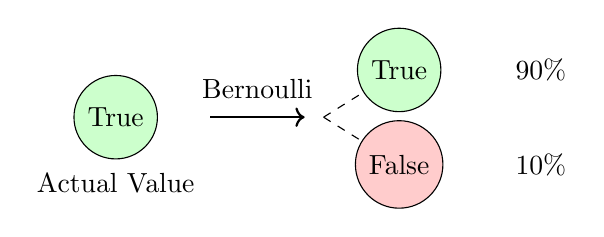
\begin{tikzpicture}[scale=1.2]
    % True value
    \node[circle,draw,fill=green!20,minimum size=1cm] (true) at (0,0) {True};
    \node at (0,-0.7) {Actual Value};
    
    % Arrow
    \draw[->,thick] (1,0) -- (2,0);
    \node at (1.5,0.3) {Bernoulli};
    
    % Possible outputs
    \node[circle,draw,fill=green!20,minimum size=1cm] (out1) at (3,0.5) {True};
    \node at (4.5,0.5) {90\%};
    
    \node[circle,draw,fill=red!20,minimum size=1cm] (out2) at (3,-0.5) {False};
    \node at (4.5,-0.5) {10\%};
    
    \draw[dashed] (2.2,0) -- (out1);
    \draw[dashed] (2.2,0) -- (out2);
\end{tikzpicture}
\end{center}

\textbf{Key Insight}: We accept occasional wrong answers in exchange for other benefits (space, privacy, speed).
\end{example}

\begin{exercise}
If you query a Bernoulli Boolean 100 times, how many correct answers do you expect? What's the probability of getting fewer than 85 correct answers?
\end{exercise}

\textit{Solution}: Expected: 90. Using binomial distribution, $P(X < 85) \approx 0.0968$.

\subsection{Visual: How Bloom Filters Work}

\begin{example}[Set Membership with False Positives]
A Bloom filter is a Bernoulli set - it can have false positives but no false negatives.

\begin{center}
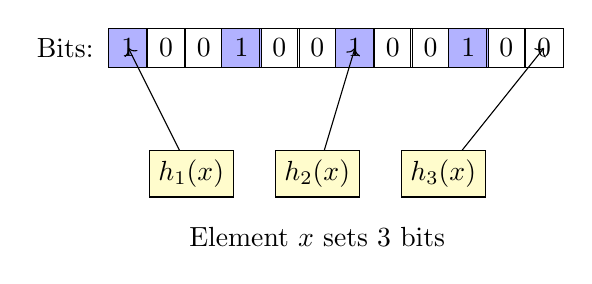
\begin{tikzpicture}[scale=0.8]
    % Bit array
    \foreach \i in {0,...,11} {
        \pgfmathtruncatemacro{\bit}{mod(\i,3)==0 ? 1 : 0}
        \ifnum\bit=1
            \node[rectangle,draw,fill=blue!30,minimum size=0.5cm] at (\i*0.6,0) {\bit};
        \else
            \node[rectangle,draw,minimum size=0.5cm] at (\i*0.6,0) {\bit};
        \fi
    }
    \node at (-1,0) {Bits:};
    
    % Hash functions
    \node[rectangle,draw,fill=yellow!20] (h1) at (1,-2) {$h_1(x)$};
    \node[rectangle,draw,fill=yellow!20] (h2) at (3,-2) {$h_2(x)$};
    \node[rectangle,draw,fill=yellow!20] (h3) at (5,-2) {$h_3(x)$};
    
    % Arrows to bits
    \draw[->] (h1) -- (0,0);
    \draw[->] (h2) -- (3.6,0);
    \draw[->] (h3) -- (6.6,0);
    
    \node at (3,-3) {Element $x$ sets 3 bits};
\end{tikzpicture}
\end{center}

To check membership: Are all 3 bits set? 
\begin{itemize}
    \item Yes $\Rightarrow$ "Probably in set" (might be false positive)
    \item No $\Rightarrow$ "Definitely not in set" (no false negatives)
\end{itemize}
\end{example}

\section{Level 2: From Approximation to Hashing}

\subsection{The Hash Construction}

\begin{example}[Encoding Values as Hash Ranges]
Instead of storing values directly, we use hash functions to create uniform representations.

\begin{center}
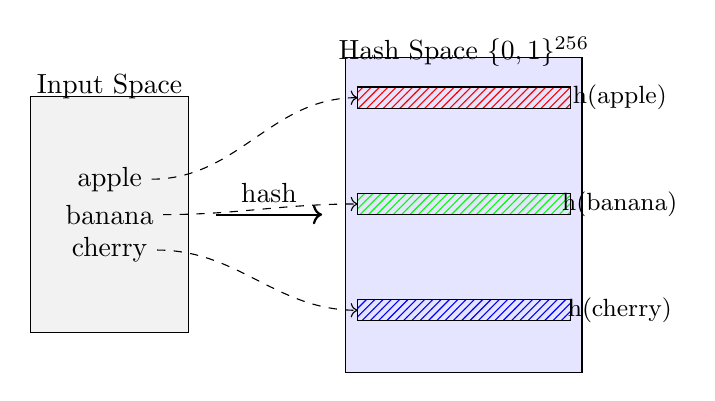
\begin{tikzpicture}[scale=0.9]
    % Input space
    \node[rectangle,draw,fill=gray!10,minimum width=2cm,minimum height=3cm] at (0,0) {};
    \node at (0,1.8) {Input Space};
    \node (a) at (0,0.5) {apple};
    \node (b) at (0,0) {banana};
    \node (c) at (0,-0.5) {cherry};
    
    % Hash function
    \draw[->,thick] (1.5,0) -- (3,0);
    \node at (2.25,0.3) {hash};
    
    % Hash space
    \node[rectangle,draw,fill=blue!10,minimum width=3cm,minimum height=4cm] at (5,0) {};
    \node at (5,2.3) {Hash Space $\{0,1\}^{256}$};
    
    % Hash outputs (visual representation)
    \draw[pattern=north east lines,pattern color=red] (3.5,1.5) rectangle (6.5,1.8);
    \node at (7.2,1.65) {\small h(apple)};
    
    \draw[pattern=north east lines,pattern color=green] (3.5,0) rectangle (6.5,0.3);
    \node at (7.2,0.15) {\small h(banana)};
    
    \draw[pattern=north east lines,pattern color=blue] (3.5,-1.5) rectangle (6.5,-1.2);
    \node at (7.2,-1.35) {\small h(cherry)};
    
    % Arrows
    \draw[dashed,->] (a) to[out=0,in=180] (3.5,1.65);
    \draw[dashed,->] (b) to[out=0,in=180] (3.5,0.15);
    \draw[dashed,->] (c) to[out=0,in=180] (3.5,-1.35);
\end{tikzpicture}
\end{center}

Each value maps to a uniform random-looking hash. No patterns in the output reveal patterns in the input.
\end{example}

\begin{exercise}
Why is uniformity important? Consider two scenarios:
\begin{enumerate}
    \item Hash outputs cluster around certain values
    \item Hash outputs are uniformly distributed
\end{enumerate}
Which reveals less information about the input distribution?
\end{exercise}

\textit{Solution}: Uniform distribution (scenario 2) reveals nothing about input patterns. Clustering would leak information about which inputs are similar or related.

\section{Level 3: Building Oblivious Functions}

\subsection{The ValidEncodings Concept}

\begin{example}[Making Functions Oblivious]
To make function $f: X \to Y$ oblivious, we define which hash values are "valid" for each output.

\begin{center}
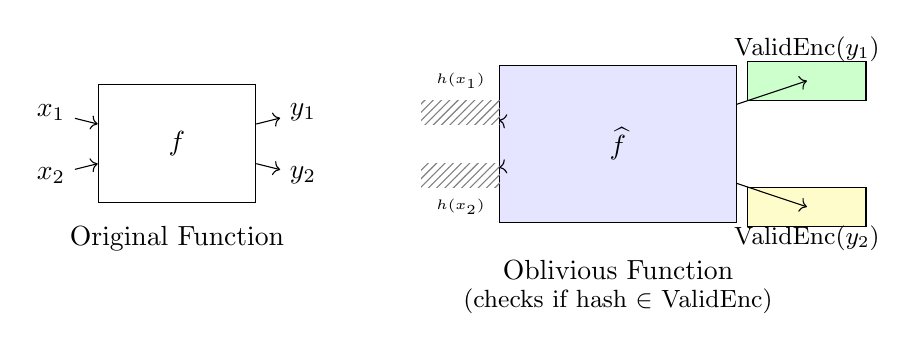
\begin{tikzpicture}[scale=0.8]
    % Function f
    \node[rectangle,draw,minimum width=2cm,minimum height=1.5cm] (f) at (0,0) {$f$};
    \node (x1) at (-2,0.5) {$x_1$};
    \node (x2) at (-2,-0.5) {$x_2$};
    \node (y1) at (2,0.5) {$y_1$};
    \node (y2) at (2,-0.5) {$y_2$};
    
    \draw[->] (x1) -- (f);
    \draw[->] (x2) -- (f);
    \draw[->] (f) -- (y1);
    \draw[->] (f) -- (y2);
    
    \node at (0,-1.5) {Original Function};
    
    % Oblivious version
    \node[rectangle,draw,fill=blue!10,minimum width=3cm,minimum height=2cm] (obv) at (7,0) {$\Obv{f}$};
    
    % Hash spaces
    \node[rectangle,pattern=north east lines,pattern color=gray,minimum width=1cm,minimum height=0.3cm] (hx1) at (4.5,0.5) {};
    \node at (4.5,1) {\tiny $h(x_1)$};
    
    \node[rectangle,pattern=north east lines,pattern color=gray,minimum width=1cm,minimum height=0.3cm] (hx2) at (4.5,-0.5) {};
    \node at (4.5,-1) {\tiny $h(x_2)$};
    
    % Valid encodings
    \node[rectangle,draw,fill=green!20,minimum width=1.5cm,minimum height=0.5cm] at (10,1) {};
    \node at (10,1.5) {\small ValidEnc($y_1$)};
    
    \node[rectangle,draw,fill=yellow!20,minimum width=1.5cm,minimum height=0.5cm] at (10,-1) {};
    \node at (10,-1.5) {\small ValidEnc($y_2$)};
    
    \draw[->] (hx1) -- (obv);
    \draw[->] (hx2) -- (obv);
    \draw[->] (obv) -- (10,1);
    \draw[->] (obv) -- (10,-1);
    
    \node at (7,-2) {Oblivious Function};
    \node at (7,-2.5) {\small (checks if hash $\in$ ValidEnc)};
\end{tikzpicture}
\end{center}
\end{example}

\subsection{Graduated Example: Building a Private Set}

\begin{example}[Step-by-Step Private Set Construction]

\textbf{Step 1: Basic Set}
\begin{verbatim}
set = {apple, banana, cherry}
contains(apple) → true
contains(grape) → false
\end{verbatim}

\textbf{Step 2: Bernoulli Set (with false positives)}
\begin{verbatim}
bloom_filter = BloomFilter(set, fp_rate=0.01)
contains(apple) → true (always correct for members)
contains(grape) → false (usually) or true (1% chance)
\end{verbatim}

\textbf{Step 3: Oblivious Set (hides membership pattern)}
\begin{verbatim}
h_apple = hash("apple" || seed)
ValidEnc_true = {0x00...0x0F}  // 1/16 of hash space
ValidEnc_false = {0x10...0xFF} // 15/16 of hash space

contains_oblivious(h_apple):
    return h_apple in ValidEnc_true
\end{verbatim}

\textbf{Step 4: Complete Oblivious System}
\begin{verbatim}
// Client encodes query
query = hash("apple" || shared_seed)

// Server checks (can't decode query)
result = oblivious_bloom_filter.contains(query)

// Client interprets result
if result in ValidEnc_true:
    print("Probably in set")
else:
    print("Not in set")
\end{verbatim}
\end{example}

\section{Level 4: Advanced Concepts}

\subsection{Tuple Encoding for Hiding Correlations}

\begin{example}[AND Queries Without Correlation Leakage]
When searching for "encryption AND backdoor", sending both terms separately reveals the correlation.

\begin{center}
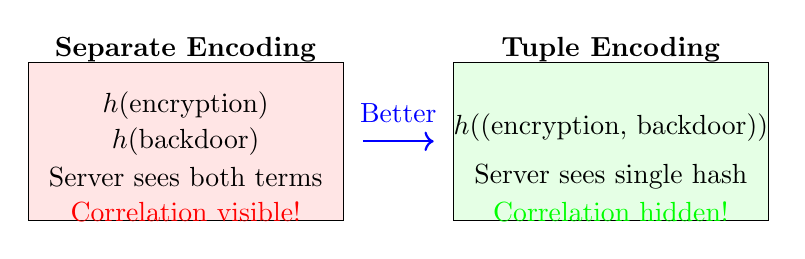
\begin{tikzpicture}[scale=0.9]
    % Separate encoding (reveals correlation)
    \node[rectangle,draw,fill=red!10,minimum width=4cm,minimum height=2cm] at (0,0) {};
    \node at (0,1.3) {\textbf{Separate Encoding}};
    \node at (0,0.5) {$h($encryption$)$};
    \node at (0,0) {$h($backdoor$)$};
    \node at (0,-0.5) {Server sees both terms};
    \node at (0,-1) {\textcolor{red}{Correlation visible!}};
    
    % Tuple encoding (hides correlation)
    \node[rectangle,draw,fill=green!10,minimum width=4cm,minimum height=2cm] at (6,0) {};
    \node at (6,1.3) {\textbf{Tuple Encoding}};
    \node at (6,0.2) {$h(($encryption, backdoor$))$};
    \node at (6,-0.5) {Server sees single hash};
    \node at (6,-1) {\textcolor{green}{Correlation hidden!}};
    
    % Arrow showing improvement
    \draw[->,thick,blue] (2.5,0) -- (3.5,0);
    \node at (3,0.4) {\textcolor{blue}{Better}};
\end{tikzpicture}
\end{center}
\end{example}

\subsection{The 1/p(x) Principle}

\begin{example}[Frequency-Based Encoding Sizes]
Common values get more encodings to hide their frequency:

\begin{center}
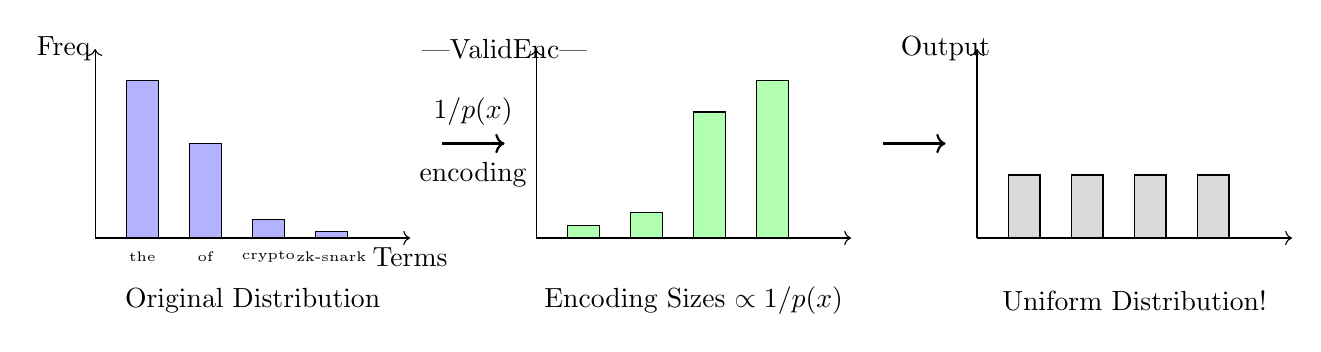
\begin{tikzpicture}[scale=0.8]
    % Frequency distribution
    \draw[->] (0,0) -- (0,3);
    \draw[->] (0,0) -- (5,0);
    \node at (-0.5,3) {Freq};
    \node at (5,-0.3) {Terms};
    
    % Original frequencies
    \draw[fill=blue!30] (0.5,0) rectangle (1,2.5);
    \node at (0.75,-0.3) {\tiny the};
    
    \draw[fill=blue!30] (1.5,0) rectangle (2,1.5);
    \node at (1.75,-0.3) {\tiny of};
    
    \draw[fill=blue!30] (2.5,0) rectangle (3,0.3);
    \node at (2.75,-0.3) {\tiny crypto};
    
    \draw[fill=blue!30] (3.5,0) rectangle (4,0.1);
    \node at (3.75,-0.3) {\tiny zk-snark};
    
    \node at (2.5,-1) {Original Distribution};
    
    % Arrow
    \draw[->,thick] (5.5,1.5) -- (6.5,1.5);
    \node at (6,2) {$1/p(x)$};
    \node at (6,1) {encoding};
    
    % Encoding sizes
    \draw[->] (7,0) -- (7,3);
    \draw[->] (7,0) -- (12,0);
    \node at (6.5,3) {|ValidEnc|};
    
    % Inverted for encoding
    \draw[fill=green!30] (7.5,0) rectangle (8,0.2);
    \draw[fill=green!30] (8.5,0) rectangle (9,0.4);
    \draw[fill=green!30] (9.5,0) rectangle (10,2);
    \draw[fill=green!30] (10.5,0) rectangle (11,2.5);
    
    \node at (9.5,-1) {Encoding Sizes $\propto 1/p(x)$};
    
    % Result
    \draw[->,thick] (12.5,1.5) -- (13.5,1.5);
    
    % Uniform output
    \draw[->] (14,0) -- (14,3);
    \draw[->] (14,0) -- (19,0);
    \node at (13.5,3) {Output};
    
    \draw[fill=gray!30] (14.5,0) rectangle (15,1);
    \draw[fill=gray!30] (15.5,0) rectangle (16,1);
    \draw[fill=gray!30] (16.5,0) rectangle (17,1);
    \draw[fill=gray!30] (17.5,0) rectangle (18,1);
    
    \node at (16.5,-1) {Uniform Distribution!};
\end{tikzpicture}
\end{center}

Rare terms need few valid encodings; common terms need many. Result: uniform observable frequency.
\end{example}

\section{Exercises with Solutions}

\subsection{Basic Exercises}

\begin{exercise}[Understanding False Positives]
You have a Bloom filter with 1000 bits and 3 hash functions, storing 100 elements. Estimate the false positive rate.
\end{exercise}

\textit{Solution}: Using the formula $p \approx (1-e^{-kn/m})^k$ where $k=3$ hash functions, $n=100$ elements, $m=1000$ bits:
\[p \approx (1-e^{-3 \cdot 100/1000})^3 = (1-e^{-0.3})^3 \approx 0.0304\]
About 3\% false positive rate.

\begin{exercise}[Hash Uniformity]
Why must hash functions produce uniform output for oblivious computing?
\end{exercise}

\textit{Solution}: Non-uniform hash output would reveal information about input distribution. If certain hash values are more common, an adversary could infer which inputs are being processed. Uniform output ensures all hash values are equally likely, hiding input patterns.

\subsection{Intermediate Exercises}

\begin{exercise}[Composing Bernoulli Functions]
If $f$ has 10\% false negatives and $g$ has 5\% false negatives, what's the error rate of $g \circ f$?
\end{exercise}

\textit{Solution}: 
\begin{itemize}
    \item Probability both correct: $(1-0.1)(1-0.05) = 0.9 \times 0.95 = 0.855$
    \item False negative rate: $1 - 0.855 = 0.145$ (14.5\%)
\end{itemize}
Note: This assumes no false positive correction. With false positives, the calculation is more complex.

\begin{exercise}[Encoding Size Calculation]
For a value appearing with probability 0.001, and another with probability 0.1, what should be the ratio of their ValidEncoding sizes to achieve uniform output?
\end{exercise}

\textit{Solution}: Using the $1/p(x)$ principle:
\[\frac{|\ValidEnc{rare}|}{|\ValidEnc{common}|} = \frac{p(common)}{p(rare)} = \frac{0.1}{0.001} = 100\]
The rare value needs 100× more valid encodings than the common value.

\subsection{Advanced Exercises}

\begin{exercise}[Security Analysis]
An adversary observes 1000 queries to an oblivious search system. What can they learn if:
\begin{enumerate}
    \item Queries use separate encoding for each term?
    \item Queries use tuple encoding for term pairs?
\end{enumerate}
\end{exercise}

\textit{Solution}:
\begin{enumerate}
    \item \textbf{Separate encoding}: Adversary learns:
        \begin{itemize}
            \item Term frequency distribution
            \item Co-occurrence patterns
            \item Temporal correlations
            \item Can potentially deduce query intent
        \end{itemize}
    \item \textbf{Tuple encoding}: Adversary learns:
        \begin{itemize}
            \item Only frequency of specific pairs (not individual terms)
            \item Cannot decompose pairs to learn about individual terms
            \item Correlation patterns are hidden
            \item Much less information leakage
        \end{itemize}
\end{enumerate}

\begin{exercise}[Implementing Oblivious AND]
Design an algorithm for oblivious AND queries that:
\begin{itemize}
    \item Hides which terms are being searched
    \item Allows false positives but not false negatives
    \item Uses tuple encoding for common pairs
\end{itemize}
\end{exercise}

\textit{Solution}:
\begin{verbatim}
class ObliviousAND:
    def __init__(self, common_pairs, threshold=0.001):
        self.pair_encodings = {}
        # Pre-compute encodings for common pairs
        for (term1, term2), freq in common_pairs.items():
            if freq > threshold:
                # Tuple encoding for common pairs
                num_encodings = int(1.0 / freq)
                self.pair_encodings[(term1,term2)] = 
                    generate_valid_encodings(num_encodings)
    
    def query(self, term1, term2):
        if (term1, term2) in self.pair_encodings:
            # Use tuple encoding
            h = hash((term1, term2))
            return h in self.pair_encodings[(term1,term2)]
        else:
            # Fall back to separate encoding
            h1 = hash(term1)
            h2 = hash(term2)
            return check_and(h1, h2)
\end{verbatim}

\section{Visual Summary: The Complete Pipeline}

\begin{center}
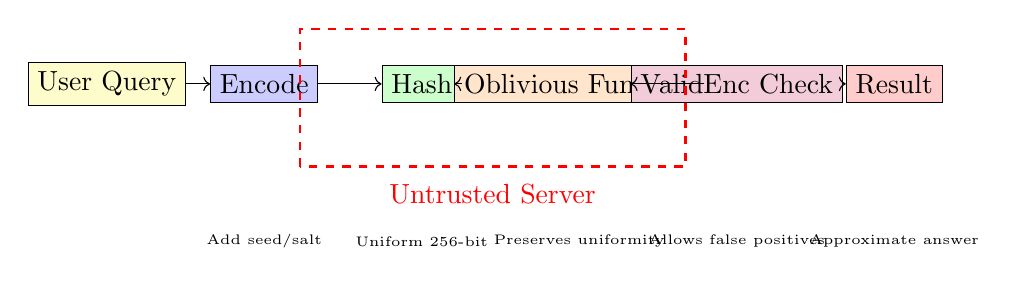
\begin{tikzpicture}[scale=0.7,node distance=2cm]
    % Nodes
    \node[rectangle,draw,fill=yellow!20] (input) {User Query};
    \node[rectangle,draw,fill=blue!20,right of=input] (encode) {Encode};
    \node[rectangle,draw,fill=green!20,right of=encode] (hash) {Hash};
    \node[rectangle,draw,fill=orange!20,right of=hash] (obv) {Oblivious Function};
    \node[rectangle,draw,fill=purple!20,right of=obv] (valid) {ValidEnc Check};
    \node[rectangle,draw,fill=red!20,right of=valid] (result) {Result};
    
    % Arrows
    \draw[->] (input) -- (encode);
    \draw[->] (encode) -- (hash);
    \draw[->] (hash) -- (obv);
    \draw[->] (obv) -- (valid);
    \draw[->] (valid) -- (result);
    
    % Annotations
    \node[below of=encode] {\tiny Add seed/salt};
    \node[below of=hash] {\tiny Uniform 256-bit};
    \node[below of=obv] {\tiny Preserves uniformity};
    \node[below of=valid] {\tiny Allows false positives};
    \node[below of=result] {\tiny Approximate answer};
    
    % Security boundary
    \draw[dashed,red,thick] (3.5,-1.5) rectangle (10.5,1);
    \node at (7,-2) {\textcolor{red}{Untrusted Server}};
\end{tikzpicture}
\end{center}

\section{Conclusion}

This pedagogical guide has taken you from basic approximation concepts to advanced oblivious computing techniques. Key takeaways:

\begin{enumerate}
    \item \textbf{Start Simple}: Understand false positives before tackling obliviousness
    \item \textbf{Build Intuition}: Visualize how hashing creates uniformity
    \item \textbf{Practice Gradually}: Work through increasingly complex examples
    \item \textbf{Connect Concepts}: See how approximation enables privacy
\end{enumerate}

\textbf{Next Steps}:
\begin{itemize}
    \item Implement a basic Bernoulli set
    \item Experiment with different encoding strategies
    \item Measure actual vs. theoretical error rates
    \item Build a simple oblivious search system
\end{itemize}

\end{document}